
\section{Theory of Relational \aclp{DB}}
\paragraph{} Brief description of basic terminology of Relational \aclp{DB}.
\begin{itemize}
	\item \textbf{Relational \acs{DB}} is a way of structuring information in tables, rows and columns with the ability to create relationships between the tables and their data.
	\item \textbf{Table} is a collection of related data stored in a table format within the database; consisting of rows and columns.
	\item \textbf{Row} or \textbf{Tuple} is a single, implicitly structured data item in a table. Every row in the table has the same structure.
	\item \textbf{Column} is a set of data values of a particular type that will hold the value for a specific information for each row.
	\item \textbf{\acl{P.K.}} is a column or a set of columns that uniquely identify each row in the table. Each table can have only one \acl{P.K.}.
	\item \textbf{\acl {F.K.}} is used to establish relationships between two entities. The \acl {F.K.} of one table is the \acl{P.K.} of another table. In some cases the \acl {F.K.} might reference the \acl{P.K.} of the same table it exists in.
\end{itemize}
\paragraph{} Small practical example of above definitions for better understanding.
\begin{figure}[h]
	\centering
	\subfloat[\centering Table: BOOK]{{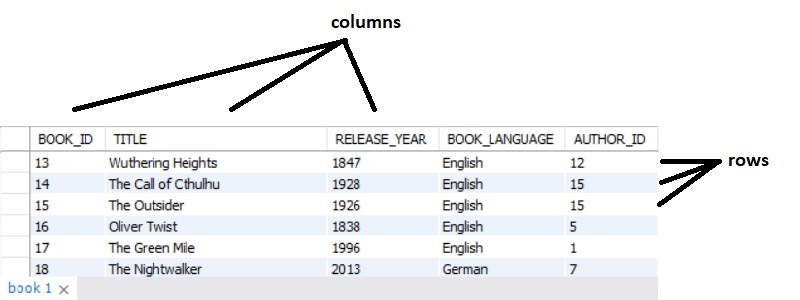
\includegraphics[width=5cm]{books-01}}}
	\qquad
	\subfloat[\centering Table: AUTHOR]{{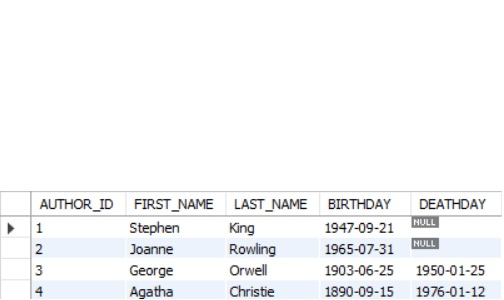
\includegraphics[width=5cm]{authors-01}}}
\end{figure}
\paragraph{} In this example in above images we have:
\begin{itemize}
	\item \textbf{Tables}: BOOK (a) and AUTHOR (b).
	\item \textbf{Rows} 6 in table BOOK and 4 in table AUTHOR. Example row: 16, Oliver Twist, 1838, English, 5.
	\item \textbf{Columns} 5 in table BOOK and 5 in table AUTHOR. Example column title in table BOOK.
	\item \textbf{\acl{P.K.}} is book\_id for table BOOK and author\_id for table AUTHOR.
	\item \textbf{\acl{F.K.}} is author\_id in table BOOK and defines which is the author for each book.
\end{itemize}
